
\documentclass[letterpaper,hide notes,xcolor={table,svgnames},pdftex,10pt]{beamer}
\def\showexamples{t}


%\usepackage[svgnames]{xcolor}

%% Demo talk
%\documentclass[letterpaper,notes=show]{beamer}

\usecolortheme{crane}
\setbeamertemplate{navigation symbols}{}

\usetheme{MyPittsburgh}
%\usetheme{Frankfurt}

%\usepackage{tipa}

\usepackage{hyperref}
\usepackage{graphicx,xspace}
\usepackage[normalem]{ulem}
\usepackage{multicol}
\usepackage{amsmath,amssymb,amsthm,graphicx,xspace}
\newcommand\SF[1]{$\bigstar$\footnote{SF: #1}}

\usepackage[default]{sourcesanspro}
\usepackage[T1]{fontenc}
\usepackage[scaled]{beramono}
\usepackage{tikzpagenodes}

\newcounter{tmpnumSlide}
\newcounter{tmpnumNote}


% old question code
%\newcommand\question[1]{{$\bigstar$ \small \onlySlide{2}{#1}}}
% \newcommand\nquestion[1]{\ifdefined \presentationonly \textcircled{?} \fi \note{\par{\Large \textbf{?}} #1}}
% \newcommand\nanswer[1]{\note{\par{\Large \textbf{A}} #1}}


 \newcommand\mnote[1]{%
   \addtocounter{tmpnumSlide}{1}
   \ifdefined\showcues {~\tiny\fbox{\arabic{tmpnumSlide}}}\fi
   \note{\setlength{\parskip}{1ex}\addtocounter{tmpnumNote}{1}\textbf{\Large \arabic{tmpnumNote}:} {#1\par}}}

\newcommand\mmnote[1]{\note{\setlength{\parskip}{1ex}#1\par}}

%\newcommand\mnote[2][]{\ifdefined\handoutwithnotes {~\tiny\fbox{#1}}\fi
% \note{\setlength{\parskip}{1ex}\textbf{\Large #1:} #2\par}}

%\newcommand\mnote[2][]{{\tiny\fbox{#1}} \note{\setlength{\parskip}{1ex}\textbf{\Large #1:} #2\par}}

\newcommand\mquestion[2]{{~\color{red}\fbox{?}}\note{\setlength{\parskip}{1ex}\par{\Large \textbf{?}} #1} \note{\setlength{\parskip}{1ex}\par{\Large \textbf{A}} #2\par}\ifdefined \presentationonly \pause \fi}

\newcommand\blackboard[1]{%
\ifdefined   \showblackboard
  {#1}
  \else {\begin{center} \fbox{\colorbox{blue!30}{%
         \begin{minipage}{.95\linewidth}%
           \hspace{\stretch{1}} Some space intentionally left blank; done at the blackboard.%
         \end{minipage}}}\end{center}}%
         \fi%
}



%\newcommand\q{\tikz \node[thick,color=black,shape=circle]{?};}
%\newcommand\q{\ifdefined \presentationonly \textcircled{?} \fi}

\usepackage{listings}
\lstset{basicstyle=\footnotesize\ttfamily,
	breaklines=true,
	aboveskip=15pt,
  	belowskip=15pt,
	frame=lines,
	numbers=left, basicstyle=\scriptsize, numberstyle=\tiny, stepnumber=0, numbersep=2pt
}

\usepackage{siunitx}
\newcommand\sius[1]{\num[group-separator = {,}]{#1}\si{\micro\second}}
\newcommand\sims[1]{\num[group-separator = {,}]{#1}\si{\milli\second}}
\newcommand\sins[1]{\num[group-separator = {,}]{#1}\si{\nano\second}}
\sisetup{group-separator = {,}, group-digits = true}

%% -------------------- tikz --------------------
\usepackage{tikz}
\usetikzlibrary{positioning}
\usetikzlibrary{arrows,backgrounds,automata,decorations.shapes,decorations.pathmorphing,decorations.markings,decorations.text,decorations.pathreplacing}

\tikzstyle{place}=[circle,draw=blue!50,fill=blue!20,thick, inner sep=0pt,minimum size=6mm]
\tikzstyle{transition}=[rectangle,draw=black!50,fill=black!20,thick, inner sep=0pt,minimum size=4mm]

\tikzstyle{block}=[rectangle,draw=black, thick, inner sep=5pt]
\tikzstyle{bullet}=[circle,draw=black, fill=black, thin, inner sep=2pt]

\tikzstyle{pre}=[<-,shorten <=1pt,>=stealth',semithick]
\tikzstyle{post}=[->,shorten >=1pt,>=stealth',semithick]
\tikzstyle{bi}=[<->,shorten >=1pt,shorten <=1pt, >=stealth',semithick]

\tikzstyle{mut}=[-,>=stealth',semithick]

\tikzstyle{treereset}=[dashed,->, shorten >=1pt,>=stealth',thin]

\usepackage{ifmtarg}
\usepackage{xifthen}
\makeatletter
% new counter to now which frame it is within the sequence
\newcounter{multiframecounter}
% initialize buffer for previously used frame title
\gdef\lastframetitle{\textit{undefined}}
% new environment for a multi-frame
\newenvironment{multiframe}[1][]{%
\ifthenelse{\isempty{#1}}{%
% if no frame title was set via optional parameter,
% only increase sequence counter by 1
\addtocounter{multiframecounter}{1}%
}{%
% new frame title has been provided, thus
% reset sequence counter to 1 and buffer frame title for later use
\setcounter{multiframecounter}{1}%
\gdef\lastframetitle{#1}%
}%
% start conventional frame environment and
% automatically set frame title followed by sequence counter
\begin{frame}%
\frametitle{\lastframetitle~{\normalfont(\arabic{multiframecounter})}}%
}{%
\end{frame}%
}
\makeatother

\makeatletter
\newdimen\tu@tmpa%
\newdimen\ydiffl%
\newdimen\xdiffl%
\newcommand\ydiff[2]{%
    \coordinate (tmpnamea) at (#1);%
    \coordinate (tmpnameb) at (#2);%
    \pgfextracty{\tu@tmpa}{\pgfpointanchor{tmpnamea}{center}}%
    \pgfextracty{\ydiffl}{\pgfpointanchor{tmpnameb}{center}}%
    \advance\ydiffl by -\tu@tmpa%
}
\newcommand\xdiff[2]{%
    \coordinate (tmpnamea) at (#1);%
    \coordinate (tmpnameb) at (#2);%
    \pgfextractx{\tu@tmpa}{\pgfpointanchor{tmpnamea}{center}}%
    \pgfextractx{\xdiffl}{\pgfpointanchor{tmpnameb}{center}}%
    \advance\xdiffl by -\tu@tmpa%
}
\makeatother
\newcommand{\copyrightbox}[3][r]{%
\begin{tikzpicture}%
\node[inner sep=0pt,minimum size=2em](ciimage){#2};
\usefont{OT1}{phv}{n}{n}\fontsize{4}{4}\selectfont
\ydiff{ciimage.south}{ciimage.north}
\xdiff{ciimage.west}{ciimage.east}
\ifthenelse{\equal{#1}{r}}{%
\node[inner sep=0pt,right=1ex of ciimage.south east,anchor=north west,rotate=90]%
{\raggedleft\color{black!50}\parbox{\the\ydiffl}{\raggedright{}#3}};%
}{%
\ifthenelse{\equal{#1}{l}}{%
\node[inner sep=0pt,right=1ex of ciimage.south west,anchor=south west,rotate=90]%
{\raggedleft\color{black!50}\parbox{\the\ydiffl}{\raggedright{}#3}};%
}{%
\node[inner sep=0pt,below=1ex of ciimage.south west,anchor=north west]%
{\raggedleft\color{black!50}\parbox{\the\xdiffl}{\raggedright{}#3}};%
}
}
\end{tikzpicture}
}


%% --------------------

%\usepackage[excludeor]{everyhook}
%\PushPreHook{par}{\setbox0=\lastbox\llap{MUH}}\box0}

%\vspace*{\stretch{1}

%\setbox0=\lastbox \llap{\textbullet\enskip}\box0}

\setlength{\parskip}{\fill}

\newcommand\noskips{\setlength{\parskip}{1ex}}
\newcommand\doskips{\setlength{\parskip}{\fill}}

\newcommand\xx{\par\vspace*{\stretch{1}}\par}
\newcommand\xxs{\par\vspace*{2ex}\par}
\newcommand\tuple[1]{\langle #1 \rangle}
\newcommand\code[1]{{\sf \footnotesize #1}}
\newcommand\ex[1]{\uline{Example:} \ifdefined \presentationonly \pause \fi
  \ifdefined\showexamples#1\xspace\else{\uline{\hspace*{2cm}}}\fi}

\newcommand\ceil[1]{\lceil #1 \rceil}


\AtBeginSection[]
{
   \begin{frame}
       \frametitle{Outline}
       \tableofcontents[currentsection]
   \end{frame}
}



\pgfdeclarelayer{edgelayer}
\pgfdeclarelayer{nodelayer}
\pgfsetlayers{edgelayer,nodelayer,main}

\tikzstyle{none}=[inner sep=0pt]
\tikzstyle{rn}=[circle,fill=Red,draw=Black,line width=0.8 pt]
\tikzstyle{gn}=[circle,fill=Lime,draw=Black,line width=0.8 pt]
\tikzstyle{yn}=[circle,fill=Yellow,draw=Black,line width=0.8 pt]
\tikzstyle{empty}=[circle,fill=White,draw=Black]
\tikzstyle{bw} = [rectangle, draw, fill=blue!20, 
    text width=4em, text centered, rounded corners, minimum height=2em]
    
    \newcommand{\CcNote}[1]{% longname
	This work is licensed under the \textit{Creative Commons #1 3.0 License}.%
}
\newcommand{\CcImageBy}[1]{%
	\includegraphics[scale=#1]{creative_commons/cc_by_30.pdf}%
}
\newcommand{\CcImageSa}[1]{%
	\includegraphics[scale=#1]{creative_commons/cc_sa_30.pdf}%
}
\newcommand{\CcImageNc}[1]{%
	\includegraphics[scale=#1]{creative_commons/cc_nc_30.pdf}%
}
\newcommand{\CcGroupBySa}[2]{% zoom, gap
	\CcImageBy{#1}\hspace*{#2}\CcImageNc{#1}\hspace*{#2}\CcImageSa{#1}%
}
\newcommand{\CcLongnameByNcSa}{Attribution-NonCommercial-ShareAlike}

\newenvironment{changemargin}[1]{% 
  \begin{list}{}{% 
    \setlength{\topsep}{0pt}% 
    \setlength{\leftmargin}{#1}% 
    \setlength{\rightmargin}{1em}
    \setlength{\listparindent}{\parindent}% 
    \setlength{\itemindent}{\parindent}% 
    \setlength{\parsep}{\parskip}% 
  }% 
  \item[]}{\end{list}} 




\title{Lecture 8 -- Asynchronous I/O, epoll, select }

\author{Patrick Lam \\ \small \texttt{p.lam@ece.uwaterloo.ca}}
\institute{Department of Electrical and Computer Engineering \\
  University of Waterloo}
\date{\today}


\begin{document}

\begin{frame}
  \titlepage

 \end{frame}

%%%%%%%%%%%%%%%%%%%%%%%%%%%%%%%%%%%%%%%%%%%%%%%%%%%%%%%%%%%%%%%%%%%%%%%%%%%%%%%%
\begin{frame}
  \frametitle{Juicy Quotes}


  \fbox{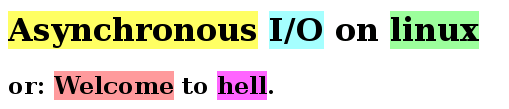
\includegraphics[width=.7\textwidth]{images/aio-linux.png}}\\
{\scriptsize (mirrored at \url{compgeom.com/~piyush/teach/4531_06/project/hell.html})}
   \\[3em]

   ``Asynchronous I/O, for example, is often infuriating.''\\
--- Robert Love. {\em Linux System Programming, 2nd ed, } page 215.
  

\end{frame}
%%%%%%%%%%%%%%%%%%%%%%%%%%%%%%%%%%%%%%%%%%%%%%%%%%%%%%%%%%%%%%%%%%%%%%%%%%%%%%%%

%%%%%%%%%%%%%%%%%%%%%%%%%%%%%%%%%%%%%%%%%%%%%%%%%%%%%%%%%%%%%%%%%%%%%%%%%%%%%%%%
\begin{frame}[fragile]
  \frametitle{Why non-blocking I/O?}
  
  Consider some I/O:


\begin{minipage}{.5\textwidth}
\begin{lstlisting}
    fd = open(...);
    read(...);
    close(fd);
  \end{lstlisting}
\end{minipage}


  Not very performant---under what conditions do we lose out?

\end{frame}
%%%%%%%%%%%%%%%%%%%%%%%%%%%%%%%%%%%%%%%%%%%%%%%%%%%%%%%%%%%%%%%%%%%%%%%%%%%%%%%%

%%%%%%%%%%%%%%%%%%%%%%%%%%%%%%%%%%%%%%%%%%%%%%%%%%%%%%%%%%%%%%%%%%%%%%%%%%%%%%%%
\begin{frame}[fragile]
  \frametitle{Mitigating I/O impact}

    So far: can use threads to mitigate latency.\\

    What are the disadvantages?
    \only<2>{
      \begin{itemize}
        \item race conditions
        \item overhead/max \# of thread limitations
      \end{itemize}
    }

\end{frame}
%%%%%%%%%%%%%%%%%%%%%%%%%%%%%%%%%%%%%%%%%%%%%%%%%%%%%%%%%%%%%%%%%%%%%%%%%%%%%%%%

%%%%%%%%%%%%%%%%%%%%%%%%%%%%%%%%%%%%%%%%%%%%%%%%%%%%%%%%%%%%%%%%%%%%%%%%%%%%%%%%
\begin{frame}
  \frametitle{Live coding: Fork Bomb! }

\begin{center}
(well, threadbomb anyway)
\end{center}

\end{frame}
%%%%%%%%%%%%%%%%%%%%%%%%%%%%%%%%%%%%%%%%%%%%%%%%%%%%%%%%%%%%%%%%%%%%%%%%%%%%%%%%

%%%%%%%%%%%%%%%%%%%%%%%%%%%%%%%%%%%%%%%%%%%%%%%%%%%%%%%%%%%%%%%%%%%%%%%%%%%%%%%%
\begin{frame}[fragile]
  \frametitle{An Alternative to Threads}

    Asynchronous/nonblocking I/O.\\[2em]


\begin{minipage}{.6\textwidth}
\begin{lstlisting}
    fd = open(..., O_NONBLOCK);
    read(...); // returns instantly!
    close(fd);
  \end{lstlisting}
\end{minipage}


\begin{center}
~\\[1em]
$\cdots$\\[2em]


\includegraphics[width=.25\textwidth]{images/Easy_button.JPG}
\end{center}
\hfill {\scriptsize (credit: Yskyflyer, Wikimedia Commons)}


\end{frame}
%%%%%%%%%%%%%%%%%%%%%%%%%%%%%%%%%%%%%%%%%%%%%%%%%%%%%%%%%%%%%%%%%%%%%%%%%%%%%%%%

%%%%%%%%%%%%%%%%%%%%%%%%%%%%%%%%%%%%%%%%%%%%%%%%%%%%%%%%%%%%%%%%%%%%%%%%%%%%%%%%
\begin{frame}
  \frametitle{Not Quite So Easy: Live Demo}

    Doesn't work on files---they're always ready. Only e.g. sockets.

\end{frame}
%%%%%%%%%%%%%%%%%%%%%%%%%%%%%%%%%%%%%%%%%%%%%%%%%%%%%%%%%%%%%%%%%%%%%%%%%%%%%%%%

%%%%%%%%%%%%%%%%%%%%%%%%%%%%%%%%%%%%%%%%%%%%%%%%%%%%%%%%%%%%%%%%%%%%%%%%%%%%%%%%
\begin{frame}
  \frametitle{Other Outstanding Problem with Nonblocking I/O}

    How do you know when I/O is ready to be queried?

    \only<2>{\begin{itemize} 
      \item polling ({\tt select}, {\tt poll}, {\tt epoll})
      \item interrupts (signals)
      \end{itemize}
    }

\end{frame}
%%%%%%%%%%%%%%%%%%%%%%%%%%%%%%%%%%%%%%%%%%%%%%%%%%%%%%%%%%%%%%%%%%%%%%%%%%%%%%%%

%%%%%%%%%%%%%%%%%%%%%%%%%%%%%%%%%%%%%%%%%%%%%%%%%%%%%%%%%%%%%%%%%%%%%%%%%%%%%%%%
\begin{frame}
  \frametitle{Using {\tt epoll}}
  
    Key idea: give {\tt epoll} a bunch of file descriptors;\\
     \hspace*{2em}wait for events to happen.\\[1em]

     Steps:
     \begin{enumerate}
       \item create an instance ({\tt epoll\_create1});
       \item populate it with file descriptors ({\tt epoll\_ctl});
       \item wait for events ({\tt epoll\_wait}).
     \end{enumerate}
  
\end{frame}
%%%%%%%%%%%%%%%%%%%%%%%%%%%%%%%%%%%%%%%%%%%%%%%%%%%%%%%%%%%%%%%%%%%%%%%%%%%%%%%%

%%%%%%%%%%%%%%%%%%%%%%%%%%%%%%%%%%%%%%%%%%%%%%%%%%%%%%%%%%%%%%%%%%%%%%%%%%%%%%%%
\begin{frame}[fragile]
  \frametitle{Creating an {\tt epoll} instance}
  
    \begin{minipage}{.5\textwidth}
    \begin{lstlisting}
   int epfd = epoll_create1(0);
    \end{lstlisting}
    \end{minipage}

    {\tt efpd} doesn't represent any files; use it to talk to {\tt epoll}.\\[1em]

    0 represents the flags (only flag: {\tt EPOLL\_CLOEXEC}).
    
  
\end{frame}
%%%%%%%%%%%%%%%%%%%%%%%%%%%%%%%%%%%%%%%%%%%%%%%%%%%%%%%%%%%%%%%%%%%%%%%%%%%%%%%%

%%%%%%%%%%%%%%%%%%%%%%%%%%%%%%%%%%%%%%%%%%%%%%%%%%%%%%%%%%%%%%%%%%%%%%%%%%%%%%%%
\begin{frame}[fragile]
  \frametitle{Populating the {\tt epoll} instance}
  
    To add {\tt fd} to the set of descriptors watched by {\tt epfd}:
    \begin{lstlisting}
   struct epoll_event event;
   int ret;
   event.data.fd = fd;
   event.events = EPOLLIN | EPOLLOUT;
   ret = epoll_ctl(epfd, EPOLL_CTL_ADD, fd, &event);
    \end{lstlisting}

    Can also modify and delete descriptors from {\tt epfd}.
  
\end{frame}
%%%%%%%%%%%%%%%%%%%%%%%%%%%%%%%%%%%%%%%%%%%%%%%%%%%%%%%%%%%%%%%%%%%%%%%%%%%%%%%%

%%%%%%%%%%%%%%%%%%%%%%%%%%%%%%%%%%%%%%%%%%%%%%%%%%%%%%%%%%%%%%%%%%%%%%%%%%%%%%%%
\begin{frame}[fragile]
  \frametitle{Waiting on an {\tt epoll} instance}
  
    Now we're ready to wait for events on any file descriptor in {\tt epfd}.
    \begin{lstlisting}
  #define MAX_EVENTS 64

  struct epoll_event events[MAX_EVENTS];
  int nr_events;

  nr_events = epoll_wait(epfd, events, MAX_EVENTS, -1);
    \end{lstlisting}

-1: wait potentially forever; otherwise, milliseconds to wait.\\[1em]

Upon return from {\tt epoll\_wait}, we have {\tt nr\_events} events ready.

  
\end{frame}
%%%%%%%%%%%%%%%%%%%%%%%%%%%%%%%%%%%%%%%%%%%%%%%%%%%%%%%%%%%%%%%%%%%%%%%%%%%%%%%%

%%%%%%%%%%%%%%%%%%%%%%%%%%%%%%%%%%%%%%%%%%%%%%%%%%%%%%%%%%%%%%%%%%%%%%%%%%%%%%%%
\begin{frame}
  \frametitle{Level-Triggered and Edge-Triggered Events}
  
    Default {\tt epoll} behaviour is \structure{level-triggered}:\\
    \quad return whenever data is ready.\\[1em]

    Can also specify (via {\tt epoll\_ctl}) \structure{edge-triggered} behaviour:\\
    \quad return whenever there is a change in readiness.\\[1em]
  
\end{frame}
%%%%%%%%%%%%%%%%%%%%%%%%%%%%%%%%%%%%%%%%%%%%%%%%%%%%%%%%%%%%%%%%%%%%%%%%%%%%%%%%


%%%%%%%%%%%%%%%%%%%%%%%%%%%%%%%%%%%%%%%%%%%%%%%%%%%%%%%%%%%%%%%%%%%%%%%%%%%%%%%%
\begin{frame}
  \frametitle{Asynchronous I/O}
  
    POSIX standard defines \structure{aio} calls.\\[1em]

    These work for disk as well as sockets.\\[1em]

    Key idea: you specify the action to occur when I/O is ready:
    \begin{itemize}
      \item nothing;
      \item start a new thread;
      \item raise a signal
    \end{itemize}

    Submit the requests using e.g. {\tt aio\_read} and {\tt aio\_write}.\\[1em]
    Can wait for I/O to happen using {\tt aio\_suspend}.
  
\end{frame}
%%%%%%%%%%%%%%%%%%%%%%%%%%%%%%%%%%%%%%%%%%%%%%%%%%%%%%%%%%%%%%%%%%%%%%%%%%%%%%%%

%%%%%%%%%%%%%%%%%%%%%%%%%%%%%%%%%%%%%%%%%%%%%%%%%%%%%%%%%%%%%%%%%%%%%%%%%%%%%%%%
\begin{frame}
  \frametitle{Nonblocking I/O with curl}
  
    Similar idea to {\tt epoll}:
\begin{itemize}
\item build up a set of descriptors;
\item invoke the transfers and wait for them to finish;
\item see how things went.
\end{itemize}
  
\end{frame}
%%%%%%%%%%%%%%%%%%%%%%%%%%%%%%%%%%%%%%%%%%%%%%%%%%%%%%%%%%%%%%%%%%%%%%%%%%%%%%%%

%%%%%%%%%%%%%%%%%%%%%%%%%%%%%%%%%%%%%%%%%%%%%%%%%%%%%%%%%%%%%%%%%%%%%%%%%%%%%%%%
\begin{frame}
  \frametitle{curl\_multi initialization}

  
    curl\_multi: work with multiple resources at once.\\[1em]

    How? Similar idea to {\tt epoll}:\\[1em]

    1. To use {\tt curl\_multi}, first create the individual requests \\ \hspace{2em} ({\tt curl\_easy\_init}).\\
    ~~~(Set options as needed on each handle).\\[1em]

    2. Then, combine them with:
    \begin{itemize}
      \item {\tt curl\_multi\_init()};
      \item {\tt curl\_multi\_add\_handle()}.
    \end{itemize}

  

\end{frame}
%%%%%%%%%%%%%%%%%%%%%%%%%%%%%%%%%%%%%%%%%%%%%%%%%%%%%%%%%%%%%%%%%%%%%%%%%%%%%%%%

%%%%%%%%%%%%%%%%%%%%%%%%%%%%%%%%%%%%%%%%%%%%%%%%%%%%%%%%%%%%%%%%%%%%%%%%%%%%%%%%
\begin{frame}
  \frametitle{curl\_multi\_perform: option 1, select-based interface}

  
    Main idea: put in requests and wait for results.\\[1em]

    {\tt curl\_multi\_perform} is a generalization of {\tt curl\_easy\_perform} to multiple resources.\\[1em]

    Handle completed transfers with {\tt curl\_multi\_info\_read}.

  

\end{frame}
%%%%%%%%%%%%%%%%%%%%%%%%%%%%%%%%%%%%%%%%%%%%%%%%%%%%%%%%%%%%%%%%%%%%%%%%%%%%%%%%

%%%%%%%%%%%%%%%%%%%%%%%%%%%%%%%%%%%%%%%%%%%%%%%%%%%%%%%%%%%%%%%%%%%%%%%%%%%%%%%%
\begin{frame}
  \frametitle{calling curl\_multi\_perform}

  
    perform interface requires use of {\tt select} (not {\tt epoll}).\\[1em]

    usage (once you've {\tt curl\_multi\_add\_handle}'d):\\[.5em]
{\tt curl\_multi\_perform(multi\_handle, \&still\_running)}\\[.5em]
    performs a non-blocking read/write, and\\
    returns the number of still-active handles\\ \hspace*{2em} (with more data to come).

  

\end{frame}
%%%%%%%%%%%%%%%%%%%%%%%%%%%%%%%%%%%%%%%%%%%%%%%%%%%%%%%%%%%%%%%%%%%%%%%%%%%%%%%%

%%%%%%%%%%%%%%%%%%%%%%%%%%%%%%%%%%%%%%%%%%%%%%%%%%%%%%%%%%%%%%%%%%%%%%%%%%%%%%%%
\begin{frame}
  \frametitle{Next steps after curl\_multi\_perform}

  
    do
    \begin{itemize}
      \item organize a call to {\tt select}; and
      \item call {\tt curl\_multi\_perform} again
    \end{itemize}
    while there are still running transfers.\\[1em]

    After the {\tt curl\_multi\_perform}, you can also delete, alter,
    and re-add an {\tt curl\_easy\_handle} when a transfer finishes.
  

\end{frame}
%%%%%%%%%%%%%%%%%%%%%%%%%%%%%%%%%%%%%%%%%%%%%%%%%%%%%%%%%%%%%%%%%%%%%%%%%%%%%%%%


%%%%%%%%%%%%%%%%%%%%%%%%%%%%%%%%%%%%%%%%%%%%%%%%%%%%%%%%%%%%%%%%%%%%%%%%%%%%%%%%
\begin{frame}[fragile]
  \frametitle{Before calling {\tt select}}

  
    {\tt select} needs a timeout and an {\tt fdset}. \\
    \qquad ({\tt curl} provides both.)\\[1em]

    Initializing the {\tt fdset} from the {\tt multi\_handle}:
  

\begin{lstlisting}
    // zero the fd-sets
    FD_ZERO(&fdread); FD_ZERO(&fdwrite); FD_ZERO(&fdexcep);
    // retrieve the fds, check for error
    curl_multi_fdset(multi_handle, 
                     &fdread, &fdwrite, &fdexcep, &maxfd);
    if (maxfd < -1) abort_("multi_fdset: couldn't wait for fds");
\end{lstlisting}

  
    Retrieving the proper timeout:
  
\begin{lstlisting}
    curl_multi_timeout(multi_handle, &curl_timeout);
\end{lstlisting}
  
    (and then convert the {\tt long} to a {\tt struct timeval}).
  

\end{frame}
%%%%%%%%%%%%%%%%%%%%%%%%%%%%%%%%%%%%%%%%%%%%%%%%%%%%%%%%%%%%%%%%%%%%%%%%%%%%%%%%

%%%%%%%%%%%%%%%%%%%%%%%%%%%%%%%%%%%%%%%%%%%%%%%%%%%%%%%%%%%%%%%%%%%%%%%%%%%%%%%%
\begin{frame}[fragile]
  \frametitle{The call to {\tt select}}

\begin{lstlisting}
  rc = select(maxfd + 1, &fdread, &fdwrite, &fdexcep, &timeout);
  if (rc == -1) abort_("[main] select error");
\end{lstlisting}

  
    Wait for one of the fds to become ready,\\ ~~or for timeout to elapse. \\[1em]
    What next?\\
    \only<2>{Call {\tt curl\_multi\_perform} again to do the work.}
  
\end{frame}
%%%%%%%%%%%%%%%%%%%%%%%%%%%%%%%%%%%%%%%%%%%%%%%%%%%%%%%%%%%%%%%%%%%%%%%%%%%%%%%%

%%%%%%%%%%%%%%%%%%%%%%%%%%%%%%%%%%%%%%%%%%%%%%%%%%%%%%%%%%%%%%%%%%%%%%%%%%%%%%%%
\begin{frame}[fragile]
  \frametitle{Knowing what happened after {\tt curl\_multi\_perform}}

  
    {\tt curl\_multi\_info\_read} will tell you.
  
\begin{lstlisting}
  msg = curl_multi_info_read(multi_handle, &msgs_left);
\end{lstlisting}
  
    and also how many messages are left.\\[1em]
    {\tt msg->msg} can be {\tt CURLMSG\_DONE} or an error;\\
    {\tt msg->easy\_handle} tells you who is done.\\[1em]
  

    Some gotchas (thanks Desiye Collier):
    \begin{itemize}
    \item Checking \verb+msg->msg == CURLMSG_DONE+ is not sufficient to ensure that a curl request actually happened. You also need to check {\tt data.result}.

    \item (A1 hint:) To reset an individual handle in the {\tt multi\_handle}, you need to ``replace'' it. But you shouldn't use {\tt curl\_easy\_init()}.  In fact, you don't need a new handle at all.
    \end{itemize}
  

\end{frame}
%%%%%%%%%%%%%%%%%%%%%%%%%%%%%%%%%%%%%%%%%%%%%%%%%%%%%%%%%%%%%%%%%%%%%%%%%%%%%%%%



%%%%%%%%%%%%%%%%%%%%%%%%%%%%%%%%%%%%%%%%%%%%%%%%%%%%%%%%%%%%%%%%%%%%%%%%%%%%%%%%
\begin{frame}
  \frametitle{curl\_multi cleanup}

  
    Call {\tt curl\_multi\_cleanup} on the multi handle.\\[1em]
    Then, call {\tt curl\_easy\_cleanup} on each easy handle.\\[2em]
    If you replace {\tt curl\_easy\_init} by {\tt curl\_global\_init},\\
    then call {\tt curl\_global\_cleanup} also.
  

\end{frame}
%%%%%%%%%%%%%%%%%%%%%%%%%%%%%%%%%%%%%%%%%%%%%%%%%%%%%%%%%%%%%%%%%%%%%%%%%%%%%%%%


%%%%%%%%%%%%%%%%%%%%%%%%%%%%%%%%%%%%%%%%%%%%%%%%%%%%%%%%%%%%%%%%%%%%%%%%%%%%%%%%
\begin{frame}
  \frametitle{curl\_multi\_perform example}

  
    Not a great example:

\begin{center}
\url{http://curl.haxx.se/libcurl/c/multi-app.html}
\end{center}

    I'm not even sure it works verbatim.\\[1em]

    Nevertheless, you could use it as a solution template.\\
    You'll have to add more code to replace completed transfers.
  

\end{frame}
%%%%%%%%%%%%%%%%%%%%%%%%%%%%%%%%%%%%%%%%%%%%%%%%%%%%%%%%%%%%%%%%%%%%%%%%%%%%%%%%

%%%%%%%%%%%%%%%%%%%%%%%%%%%%%%%%%%%%%%%%%%%%%%%%%%%%%%%%%%%%%%%%%%%%%%%%%%%%%%%%
\begin{frame}
  \frametitle{A better choice: curl\_multi\_wait}

  
    Instead of using {\tt select()}, \\
    you can use {\tt curl\_multi\_wait()}.\\[2em]
    It's just better.\\
  \url{https://gist.github.com/clemensg/4960504}
  
\end{frame}
%%%%%%%%%%%%%%%%%%%%%%%%%%%%%%%%%%%%%%%%%%%%%%%%%%%%%%%%%%%%%%%%%%%%%%%%%%%%%%%%

%%%%%%%%%%%%%%%%%%%%%%%%%%%%%%%%%%%%%%%%%%%%%%%%%%%%%%%%%%%%%%%%%%%%%%%%%%%%%%%%
\begin{frame}
  \frametitle{curl\_multi, option 3: curl\_multi\_socket\_action}

  
    So, I couldn't quite figure out how this works. Sorry.\\[1em]

    Similar to the {\tt perform} interface, but you have more control.

    Advantage:

\begin{quote}
   2 - When the application discovers action on a single socket, it calls
       libcurl and informs that there was action on this particular socket and
       libcurl can then act on that socket/transfer only and not care about
       any other transfers. (The previous API always had to scan through all
       the existing transfers.)
\end{quote}

\url{http://curl.haxx.se/dev/readme-multi_socket.html}

  
\end{frame}
%%%%%%%%%%%%%%%%%%%%%%%%%%%%%%%%%%%%%%%%%%%%%%%%%%%%%%%%%%%%%%%%%%%%%%%%%%%%%%%%

%%%%%%%%%%%%%%%%%%%%%%%%%%%%%%%%%%%%%%%%%%%%%%%%%%%%%%%%%%%%%%%%%%%%%%%%%%%%%%%%
\begin{frame}

  \frametitle{multi\_socket usage}


From the manpage:
\small
\begin{itemize}
\item Create a multi handle

\item Set the socket callback with {\tt CURLMOPT\_SOCKETFUNCTION}

\item Set the timeout callback with {\tt CURLMOPT\_TIMERFUNCTION}, to get to know what timeout value to use when waiting for socket activities.

\item Add easy handles with {\tt curl\_multi\_add\_handle()}

\item Provide some means to manage the sockets libcurl is using, so you can check them for activity. This can be done through your application code, or by way of an external library such as libevent or glib.

\item Call {\tt curl\_multi\_socket\_action(..., CURL\_SOCKET\_TIMEOUT, 0, ...)} to kickstart everything. To get one or more callbacks called.

\item Wait for activity on any of libcurl's sockets, use the timeout value your callback has been told.

\item When activity is detected, call {\tt curl\_multi\_socket\_action()} for the socket(s) that got action. If no activity is detected and the timeout expires, call {\tt curl\_multi\_socket\_action(3)} with {\tt CURL\_SOCKET\_TIMEOUT}. 
\end{itemize}
  

\end{frame}
%%%%%%%%%%%%%%%%%%%%%%%%%%%%%%%%%%%%%%%%%%%%%%%%%%%%%%%%%%%%%%%%%%%%%%%%%%%%%%%%

%%%%%%%%%%%%%%%%%%%%%%%%%%%%%%%%%%%%%%%%%%%%%%%%%%%%%%%%%%%%%%%%%%%%%%%%%%%%%%%%
\begin{frame}

  \frametitle{multi\_socket example}


This example is even worse than the last one:
\begin{center}
\url{http://curl.haxx.se/libcurl/c/hiperfifo.html}
\end{center}~\\[1em]
It contains more moving parts than we need to understand the API, and gets
another library ({\tt libevent}) involved.

\end{frame}
%%%%%%%%%%%%%%%%%%%%%%%%%%%%%%%%%%%%%%%%%%%%%%%%%%%%%%%%%%%%%%%%%%%%%%%%%%%%%%%%

%%%%%%%%%%%%%%%%%%%%%%%%%%%%%%%%%%%%%%%%%%%%%%%%%%%%%%%%%%%%%%%%%%%%%%%%%%%%%%%%
\begin{frame}
  \frametitle{Concurrent Socket I/O}

  
    Complete change of topic. A Quora question:

    \begin{quote}
      What is the ideal design for server process in Linux that handles concurrent socket I/O?
    \end{quote}

    So far in this class, we've seen:
    \begin{itemize}
    \item processes;
    \item threads;
    \item thread pools; and
      \item async/non-blocking I/O.
    \end{itemize}

    We'll see the answer by Robert Love, Linux kernel hacker\footnote{\tiny \url{https://plus.google.com/105706754763991756749/posts/VPMT8ucAcFH}}.

  
\end{frame}
%%%%%%%%%%%%%%%%%%%%%%%%%%%%%%%%%%%%%%%%%%%%%%%%%%%%%%%%%%%%%%%%%%%%%%%%%%%%%%%%

%%%%%%%%%%%%%%%%%%%%%%%%%%%%%%%%%%%%%%%%%%%%%%%%%%%%%%%%%%%%%%%%%%%%%%%%%%%%%%%%
\begin{frame}
  \frametitle{The Real Question}

  
    \Large
    \begin{quote}
      How do you want to do I/O?\\[1em]
    \end{quote}

    Not really ``how many threads?''.
  

\end{frame}
%%%%%%%%%%%%%%%%%%%%%%%%%%%%%%%%%%%%%%%%%%%%%%%%%%%%%%%%%%%%%%%%%%%%%%%%%%%%%%%%

%%%%%%%%%%%%%%%%%%%%%%%%%%%%%%%%%%%%%%%%%%%%%%%%%%%%%%%%%%%%%%%%%%%%%%%%%%%%%%%%
\begin{frame}
  \frametitle{Four Choices}

  
    \begin{itemize}
      \item Blocking I/O; 1 process per request.
      \item Blocking I/O; 1 thread per request.
      \item Asynchronous I/O, pool of threads, \\callbacks, \\ each thread handles multiple connections.
      \item Nonblocking I/O, pool of threads, \\ multiplexed with select/poll,
        event-driven, \\ each thread handles multiple connections.
    \end{itemize}
  

\end{frame}
%%%%%%%%%%%%%%%%%%%%%%%%%%%%%%%%%%%%%%%%%%%%%%%%%%%%%%%%%%%%%%%%%%%%%%%%%%%%%%%%

%%%%%%%%%%%%%%%%%%%%%%%%%%%%%%%%%%%%%%%%%%%%%%%%%%%%%%%%%%%%%%%%%%%%%%%%%%%%%%%%
\begin{frame}
  \frametitle{Blocking I/O; 1 process per request}

  
  Old Apache model: \hfill 
\includegraphics[width=.2\textwidth]{images/httpd_logo_wide_new}

  \begin{itemize}
    \item Main thread waits for connections.
    \item Upon connect, forks off a new process, \\which completely
      handles the connection.
    \item Each I/O request is blocking: \\ e.g. reads wait until more data arrives.
  \end{itemize}

  Advantage: 
  \begin{itemize}
    \item ``Simple to undertand and easy to program.''
  \end{itemize}

  Disadvantage:
  \begin{itemize}
    \item High overhead from starting 1000s of processes.\\
      (can somewhat mitigate with process pool).
  \end{itemize}
  Can handle $\sim$10 000 processes, but doesn't generally scale.

  

\end{frame}
%%%%%%%%%%%%%%%%%%%%%%%%%%%%%%%%%%%%%%%%%%%%%%%%%%%%%%%%%%%%%%%%%%%%%%%%%%%%%%%%

%%%%%%%%%%%%%%%%%%%%%%%%%%%%%%%%%%%%%%%%%%%%%%%%%%%%%%%%%%%%%%%%%%%%%%%%%%%%%%%%
\begin{frame}
  \frametitle{Blocking I/O; 1 thread per request}

  
    We know that threads are more lightweight than processes.\\[1em]

    Same as 1 process per request, but less overhead.\\[1em]

    I/O is the same---still blocking.\\[1em]

    Advantage:
    \begin{itemize}
      \item Still simple to understand and easy to program.
    \end{itemize}

    Disadvantages:
    \begin{itemize}
      \item Overhead still piles up, although less than processes.
      \item New complication: race conditions on shared data.
    \end{itemize}
  
\end{frame}
%%%%%%%%%%%%%%%%%%%%%%%%%%%%%%%%%%%%%%%%%%%%%%%%%%%%%%%%%%%%%%%%%%%%%%%%%%%%%%%%

%%%%%%%%%%%%%%%%%%%%%%%%%%%%%%%%%%%%%%%%%%%%%%%%%%%%%%%%%%%%%%%%%%%%%%%%%%%%%%%%
\begin{frame}
  \frametitle{Asynchronous I/O Benefits}

  
    In 2006, perf benefits of asynchronous I/O on lighttpd\footnote{\tiny \url{http://blog.lighttpd.net/articles/2006/11/12/lighty-1-5-0-and-linux-aio/}}:\\

{\small
    \begin{tabular}{llrrr}
    version & & fetches/sec & bytes/sec & CPU idle \\
    1.4.13 & sendfile & 36.45 & 3.73e+06 & 16.43\% \\
    1.5.0 & sendfile & 40.51 & 4.14e+06 & 12.77\% \\
    1.5.0 & linux-aio-sendfile & 72.70 & 7.44e+06 & 46.11\% \\
    \end{tabular}
}~\\[1em]

    (Workload: $2\times 7200$ RPM in RAID1, 1GB RAM, \\
     \qquad transferring 10GBytes on a 100MBit network).\\[1em]
  
\end{frame}
%%%%%%%%%%%%%%%%%%%%%%%%%%%%%%%%%%%%%%%%%%%%%%%%%%%%%%%%%%%%%%%%%%%%%%%%%%%%%%%%

%%%%%%%%%%%%%%%%%%%%%%%%%%%%%%%%%%%%%%%%%%%%%%%%%%%%%%%%%%%%%%%%%%%%%%%%%%%%%%%%
\begin{frame}
  \frametitle{Using Asynchronous I/O in Linux (select/poll)}


   Basic workflow: \\[1em]
   \begin{enumerate}
     \item enqueue a request;
     \item \ldots ~do something else;
     \item (if needed) periodically check whether request is done; and
     \item read the return value.
   \end{enumerate}

  
\end{frame}
%%%%%%%%%%%%%%%%%%%%%%%%%%%%%%%%%%%%%%%%%%%%%%%%%%%%%%%%%%%%%%%%%%%%%%%%%%%%%%%%

%%%%%%%%%%%%%%%%%%%%%%%%%%%%%%%%%%%%%%%%%%%%%%%%%%%%%%%%%%%%%%%%%%%%%%%%%%%%%%%%
\begin{frame}[fragile]
  \frametitle{Asynchronous I/O Code Example I: Setup}

  
\begin{lstlisting}
#include <aio.h>

int main() {
    // so far, just like normal
    int file = open("blah.txt", O_RDONLY, 0);

    // create buffer and control block
    char* buffer = new char[SIZE_TO_READ];
    aiocb cb;
    
    memset(&cb, 0, sizeof(aiocb));
    cb.aio_nbytes = SIZE_TO_READ;
    cb.aio_fildes = file;
    cb.aio_offset = 0;
    cb.aio_buf = buffer;
\end{lstlisting}
  

\end{frame}
%%%%%%%%%%%%%%%%%%%%%%%%%%%%%%%%%%%%%%%%%%%%%%%%%%%%%%%%%%%%%%%%%%%%%%%%%%%%%%%%

%%%%%%%%%%%%%%%%%%%%%%%%%%%%%%%%%%%%%%%%%%%%%%%%%%%%%%%%%%%%%%%%%%%%%%%%%%%%%%%%
\begin{frame}[fragile]
  \frametitle{Asynchronous I/O Code Example II: Read}

  
\begin{lstlisting}
    // enqueue the read
    if (aio_read(&cb) == -1) { /* error handling */ }

    do {
      // ... do something else ...
    while (aio_error(&cb) == EINPROGRESS); // poll

    // inspect the return value
    int numBytes = aio_return(&cb);
    if (numBytes == -1) { /* error handling */ }

    // clean up
    delete[] buffer;
    close(file);
\end{lstlisting}
  
\end{frame}

%%%%%%%%%%%%%%%%%%%%%%%%%%%%%%%%%%%%%%%%%%%%%%%%%%%%%%%%%%%%%%%%%%%%%%%%%%%%%%%%
\begin{frame}
  \frametitle{Nonblocking I/O in Servers using Select/Poll}

  
    Each thread handles multiple connections.\\[1em]

    When a thread is ready, it uses select/poll to find work.\\

    \begin{itemize}
      \item perhaps it needs to read from disk into a mmap'd tempfile;
      \item perhaps it needs to copy the tempfile to the network.
    \end{itemize}~\\
    In either case, the thread does work and updates the request state.
  
\end{frame}
%%%%%%%%%%%%%%%%%%%%%%%%%%%%%%%%%%%%%%%%%%%%%%%%%%%%%%%%%%%%%%%%%%%%%%%%%%%%%%%%

%%%%%%%%%%%%%%%%%%%%%%%%%%%%%%%%%%%%%%%%%%%%%%%%%%%%%%%%%%%%%%%%%%%%%%%%%%%%%%%%
\begin{frame}
  \frametitle{Callback-Based Asynchronous I/O Model}

  
    Weird programming model; not popular.\\[1em]
    Instead of select/poll, pass along a callback,\\ to be executed upon success or failure.\\[1em]
    JavaScript does this extensively, but more unwieldy in C.\\[1em]
    We'll see the Go programming model, which makes this easy.
  
\end{frame}
%%%%%%%%%%%%%%%%%%%%%%%%%%%%%%%%%%%%%%%%%%%%%%%%%%%%%%%%%%%%%%%%%%%%%%%%%%%%%%%%

%%%%%%%%%%%%%%%%%%%%%%%%%%%%%%%%%%%%%%%%%%%%%%%%%%%%%%%%%%%%%%%%%%%%%%%%%%%%%%%%
\begin{frame}[fragile]
  \frametitle{Callback-Based Example}

\begin{lstlisting}
void
new_connection_cb (int cfd)
{
  if (cfd < 0) {
    fprintf (stderr, "error in accepting connection!\n");
    exit (1);
  }

  ref<connection_state> c = 
    new refcounted<connection_state>(cfd);

  c->killing_task = delaycb(10, 0, wrap(&clean_up, c));

  /* next step: read information on the new connection */
  fdcb (cfd, selread, wrap (&read_http_cb, cfd, c, true,
                 wrap(&read_req_complete_cb)));
}
\end{lstlisting}

\end{frame}
%%%%%%%%%%%%%%%%%%%%%%%%%%%%%%%%%%%%%%%%%%%%%%%%%%%%%%%%%%%%%%%%%%%%%%%%%%%%%%%%

%%%%%%%%%%%%%%%%%%%%%%%%%%%%%%%%%%%%%%%%%%%%%%%%%%%%%%%%%%%%%%%%%%%%%%%%%%%%%%%%
\begin{frame}[fragile]
  \frametitle{node.js: A Superficial View}

   node.js is another event-based nonblocking I/O model.\\[1em]

   (Since JavaScript is singlethreaded, nonblocking I/O mandatory.)\\[1em]

Canonical example from node.js homepage:
\begin{lstlisting}
var http = require('http');
http.createServer(function (req, res) {
  res.writeHead(200, {'Content-Type': 'text/plain'});
  res.end('Hello World\n');
}).listen(1337, '127.0.0.1');
console.log('Server running at http://127.0.0.1:1337/');
\end{lstlisting}

Note the use of the callback---it's called upon each connection.

\end{frame}
%%%%%%%%%%%%%%%%%%%%%%%%%%%%%%%%%%%%%%%%%%%%%%%%%%%%%%%%%%%%%%%%%%%%%%%%%%%%%%%%

%%%%%%%%%%%%%%%%%%%%%%%%%%%%%%%%%%%%%%%%%%%%%%%%%%%%%%%%%%%%%%%%%%%%%%%%%%%%%%%%
\begin{frame}[fragile]
  \frametitle{Building on node.js}

Usually we want a higher-level view, e.g. expressjs\footnote{\url{http://expressjs.com}}.\\[1em]

An example from the Internet\footnote{\tiny \url{https://github.com/tglines/nodrr/blob/master/controllers/nod.js}}:
\begin{lstlisting}
app.post('/nod', function(req, res) {
  loadAccount(req,function(account) {
    if(account && account.username) {
      var n = new Nod();
      n.username = account.username;
      n.text = req.body.nod;
      n.date = new Date();
      n.save(function(err){
        res.redirect('/');
      });
    }
  });
});
\end{lstlisting}

\end{frame}
%%%%%%%%%%%%%%%%%%%%%%%%%%%%%%%%%%%%%%%%%%%%%%%%%%%%%%%%%%%%%%%%%%%%%%%%%%%%%%%%

%%%%%%%%%%%%%%%%%%%%%%%%%%%%%%%%%%%%%%%%%%%%%%%%%%%%%%%%%%%%%%%%%%%%%%%%%%%%%%%%
\begin{frame}
  \frametitle{Summary: Building Servers}

  
    \begin{itemize}
      \item Blocking I/O; 1 process per request (old Apache).
      \item Blocking I/O; 1 thread per request (Java).
      \item Asynchronous I/O, pool of threads, callbacks, \\ each thread handles multiple connections. (no one does this)
      \item Nonblocking I/O, pool of threads, \\ multiplexed with select/poll,
        event-driven, \\ each thread handles multiple connections. (JavaScript)
    \end{itemize}
  

\end{frame}
%%%%%%%%%%%%%%%%%%%%%%%%%%%%%%%%%%%%%%%%%%%%%%%%%%%%%%%%%%%%%%%%%%%%%%%%%%%%%%%%

\end{document}

